\chapter{Statistical Inference}

\section{Classical Parameter Estimation}

Consider a set of observations/data $\{(x_1, y_1), (x_2, y_2), \dots, (x_n, y_n)\},$ and let $\mathbf{\Theta}$ be a set of $k$ parameters. $x_i\in\mathcal{X}$ is the index (usually something like time) of each observation. We assume that $\mathbf\Theta\in\mathbb{R}^k.$

Let $\hat{y}\left(x_i | \mathbf{\Theta}\right)$ be a function mapping to $\mathbb{R}.$ Under the frequentist interpretation, $\mathbf\Theta$ is fixed, and does not have any underlying distribution. This section explores ways to estimate $\mathbf\Theta$ under this assumption.

\subsection*{Least Squares Estimator}

The least squares estimate $\mathbf{\Theta}_{\mathrm{LS}}$ of the set of parameters $\mathbf{\Theta}$ is defined as $$\mathbf{\Theta}_{\mathrm{LS}} := \argmin_{\mathbf{\Theta}} \sum_{i = 1}^n (\hat{y}\left(x_i | \mathbf{\Theta}\right)- y_i)^2.$$

For example, if we had a set of data $\{(1, 2), (2, 4), (3, 4)\},$ and $\mathbf\Theta = \{a, b\}.$ We consider a linear model $$\hat{y}\left(x_i|a, b\right) = a + bx_i.$$ Therefore
\begin{align*}
    \mathbf{\Theta}_{\mathrm{LS}} =&\, \argmin_{a, b} \sum_{i = 1}^4 (a + bx_i - y_i)^2\\
    =&\, \argmin_{a, b} (a + b - 2)^2 + (a + 2b - 4)^2 + (a + 3b - 4)^2 + (a + 4b - 7)^2
\end{align*} and so we consider
\begin{align*}
    0 =&\, \frac{\partial}{\partial a} (a + b - 2)^2 + (a + 2b - 4)^2 + (a + 3b - 4)^2\\
    =&\, 2(a + b - 2 + a + 2b - 4 + a + 3b - 4)\\
    =&\, 2(3a + 6b - 10)\\
    \implies a =&\, \frac{10}{3} - 2b
\end{align*} and
\begin{align*}
    0 =&\, \frac{\partial}{\partial b} (a + b - 2)^2 + (a + 2b - 4)^2 + (a + 3b - 4)^2\\
    =&\, 2(a + b - 2) + 4(a + 2b - 4) + 6(a + 3b - 4)\\
    =&\, 2(a + b - 2 + 2a + 4b - 8 + 3a + 9b - 12)\\
    =&\, 4(3a + 7b - 11)\\
    \implies a =&\, \frac{11}{3} - \frac{7b}{3}.
\end{align*} Combining these we have
\begin{align*}
    \frac{10}{3} - 2b =&\, \frac{11}{3} - \frac{7b}{3}\\
    \implies 10 - 6b =&\, 11 - 7b\\
    \implies b =&\, 1\\
    \implies a =&\, \frac{10}{3} - 2 = 4/3
\end{align*}

\subsection*{Maximum Likelihood Estimator}

The least square method makes no explicit assumptions about what distribution $y_i$ is generated from, and only informs a deterministic model. However if we know (or in reality can make a reasonable assumption of) the distribution that the observations are from, we can instead use the likelihood to estimate the parameters. This is a very standard frequentist approach.

\todo{discuss the general case here}

For the data in figure \ref{fig:LSE} if $y_i \sim \mathrm{Pois}(a + bx_i),$ we can find the maximum likelihood estimators $(\hat{a}, \hat{b})$ by
\begin{align*}
    (\hat{a}, \hat{b}) =& \argmax_{a, b}\prod_{i = 1}^{4} \frac{(a + bx_i)^{y_i}\exp(-a - bx_i)}{y_i!}\\
    =&\, \argmax_{a, b} \sum_{i = 1}^{4} y_i\ln(a + bx_i) - a - bx_i - \ln(y_i!)\tag{by the monotonicity of $\ln(x)$}\\
    =&\, \argmax_{a, b} 2\ln(a + b) - a - b + 4\ln(a + 2b) - a - b + 4\ln(a + 3b) - a - b\\
    =&\, \argmax_{a, b} 2\ln(a + b) + 4\ln(a + 2b) + 4\ln(a + 3b) - 4a - 4b.
\end{align*} This is a non-convex function, and so we numerically solve to find a maximum. We get $\hat{a} \approx 1.329$ and $\hat{b} \approx 0.751$ as seen in figure \ref{fig:LSE}.

\begin{figure}[ht]
    \centering
    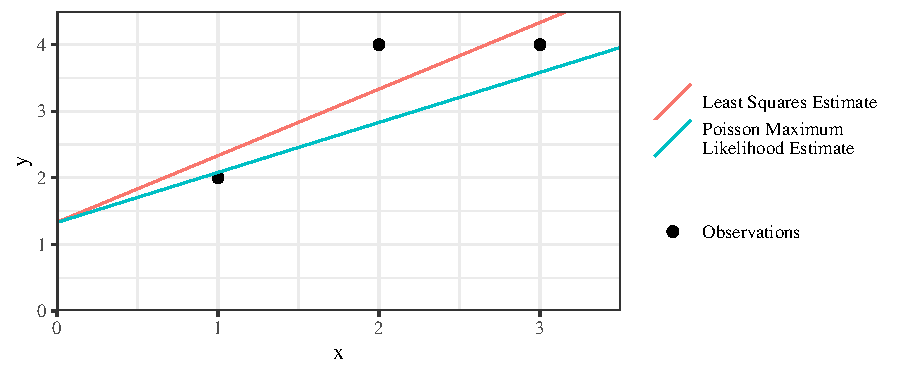
\includegraphics{LS_example.pdf}
    \caption{Two linear models of the form $y = a + bx$ were fit given the set of observations $\{(1, 2), (2, 4), (3, 4)\}$ using least squares estimators for $a$ and $b,$ and the maximum likelihood estimators under the assumption that the data are independent realisations by a Poisson distribution with $\lambda = y.$}
    \label{fig:LSE}
\end{figure}

\subsection*{Relationship Between the Least Squares and Maximum Likelihood Estimators}

If each realisation of the data is normally distributed with equal variance $\sigma^2$ (i.e. $y_i \sim N(y_i|\mu_i(\mathbf{\Theta}), \sigma^2)$) then the maximum likelihood estimator of $\mathbf{\Theta}$ (the set of parameters) is
\begin{align*}
    \argmax_{\mathbf{\Theta}}\mathcal{L}(\mathbf{\Theta}) =&\, \argmax_{\mathbf{\Theta}} \prod_{i = 1}^n \frac{1}{\sqrt{2\pi}\sigma}\exp\left(-\frac{(\hat{y}\left(x_i | \mathbf{\Theta}\right)- y_i)^2}{\sigma^2}\right)\\
    =& \argmax_{\mathbf{\Theta}} \sum_{i = 1}^n \ln\left(\frac{1}{\sqrt{2\pi}\sigma}\right) - \frac{(\hat{y}\left(x_i | \mathbf{\Theta}\right)- y_i)^2}{\sigma^2}\\
    =& \argmax_{\mathbf{\Theta}} \sum_{i = 1}^n - (\hat{y}\left(x_i | \mathbf{\Theta}\right)- y_i)^2\\
    =& \argmin_{\mathbf{\Theta}} \sum_{i = 1}^n (\hat{y}\left(x_i | \mathbf{\Theta}\right)- y_i)^2
\end{align*}
which is exactly the least squares estimator.

